%%%%%%%%%%%%%%%%%%%%%%%%%%%%%%%%%%%%%%%%%%%%%%%%%%%%%%%%%%%%%%%%%%%%%%%%%%%%%%%%%%%%%%%%%%%%%%%%%%%%%%%%%%%%%%%%%%%%%%%%%%%%%%%%%%%%%%%%%%%%%%%%%%%%%%%%%%%%%%%%%%%%%%%%%%%%%%%%%%%%%%%%%%%%
% Written By Michael Brodskiy
% Club: Science Bowl/Olympiad
%%%%%%%%%%%%%%%%%%%%%%%%%%%%%%%%%%%%%%%%%%%%%%%%%%%%%%%%%%%%%%%%%%%%%%%%%%%%%%%%%%%%%%%%%%%%%%%%%%%%%%%%%%%%%%%%%%%%%%%%%%%%%%%%%%%%%%%%%%%%%%%%%%%%%%%%%%%%%%%%%%%%%%%%%%%%%%%%%%%%%%%%%%%%

\documentclass[12pt]{article} 
\usepackage{alphalph}
\usepackage[utf8]{inputenc}
\usepackage[russian,english]{babel}
\usepackage{titling}
\usepackage{amsmath}
\usepackage{graphicx}
\usepackage{enumitem}
\usepackage{amssymb}
\usepackage[super]{nth}
\usepackage{everysel}
\usepackage{ragged2e}
\usepackage{geometry}
\usepackage{multicol}
\usepackage{fancyhdr}
\usepackage{cancel}
\usepackage{siunitx}
\usepackage{wrapfig}
\geometry{top=1.0in,bottom=1.0in,left=1.0in,right=1.0in}
\newcommand{\subtitle}[1]{%
  \posttitle{%
    \par\end{center}
    \begin{center}\large#1\end{center}
    \vskip0.5em}%

}
\usepackage{hyperref}
\hypersetup{
colorlinks=true,
linkcolor=blue,
filecolor=magenta,      
urlcolor=blue,
citecolor=blue,
}

\urlstyle{same}
\usepackage{fancyhdr}
\pagestyle{fancy}
\lhead[\textsc{Las Lomas HS}]{\textsc{Las Lomas HS}}
\chead[\textsc{Science Bowl \& Olympiad Journal}]{\textsc{Science Bowl \& Olympiad Journal}}
\rhead[\textsc{\copyright 2020—2021}]{\textsc{\copyright 2020—2021}}
\cfoot[]{}


% Mathematical Operations:

% Sum: $$\sum_{n=a}^{b} f(x) $$
% Integral: $$\int_{lower}^{upper} f(x) dx$$
% Limit: $$\lim_{x\to\infty} f(x)$$

\begin{document}

\begin{center}
  
\includegraphics[width=.9\textwidth]{Images/FSFLogo.png}
\end{center}

\begin{multicols}{3}

  With a rise in the prevalence and complexity of technology, come questions on the ethics. These questions range from privacy and tracking protection to whether companies should be able to proprietize, and therefore obfuscate, their products. The underlying argument of the Free Software Foundation, abbreviated FSF, essentially lies in a dichotomy: if the user does not control their system, then the system controls them. Nowadays, companies such as Microsoft, Google, Apple, and many more profit off of clueless users by forcing them to pay, perpetually, not for the product, but for a license to be able to use said product. This immoral business model limits the users' ability to properly use the software, thereby dividing the user community and establishing the dominance of the company over the user. Richard Stallman (RMS), the chief GNUisance and founder of the FSF, has been fighting for the rights of users since the early 1970s, when he graduated with a degree in physics from Harvard University, and joined the MIT Artificial Intelligence Laboratory.  Stallman argues that, for a piece of software to be free (that is, free as in freedom, not price), it must follow the four freedoms: first (or the zeroth term, the way Stallman numbers it), a user must be able to run the program for any purpose. Second, a user must be able to study the program and change it to their needs. Third, a user must be able to redistribute the program to help out their neighbor. Finally, fourth, a user must be able to improve the program, and release said improvements to other members of the community. 

  \vfill

  \begin{wrapfigure}{l}{.6\linewidth}
  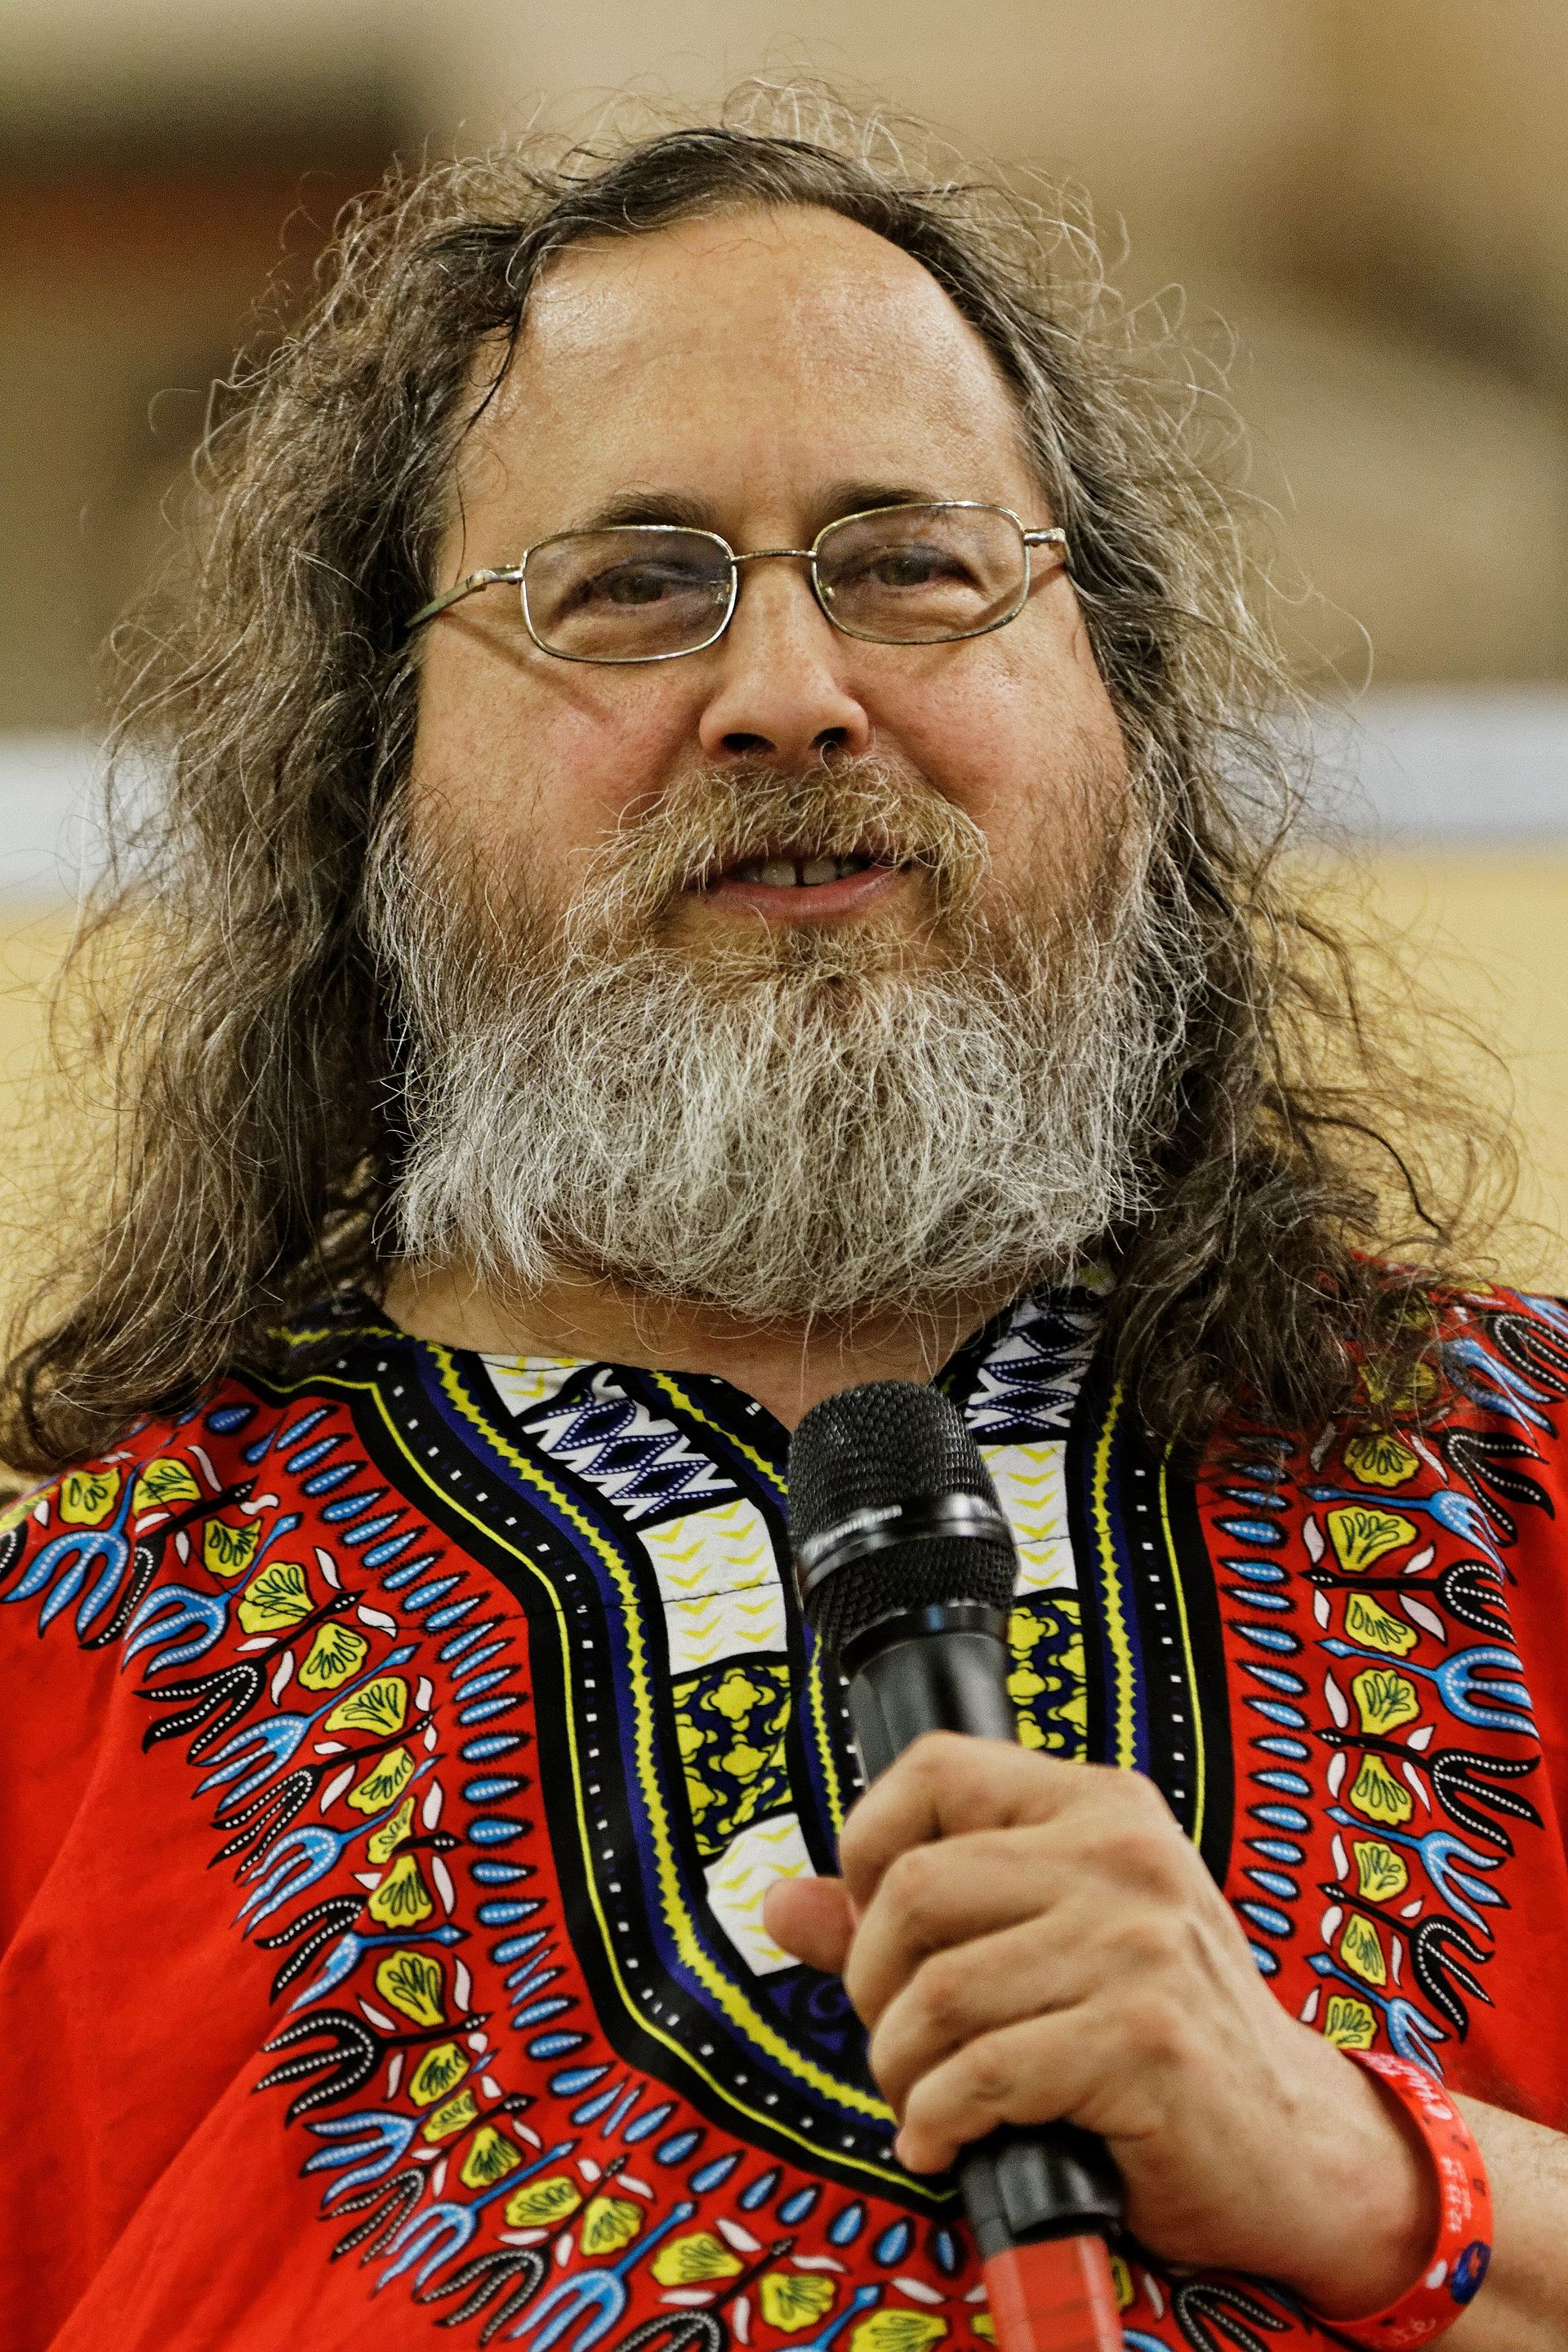
\includegraphics[width=\linewidth]{Images/Stallman.jpeg}
  \end{wrapfigure}

  \vfill

  Now with codified requirements, Stallman set out to create a license to benefit the community. This was established as the GPL, or General Public License, which has since reached the third version. Of course, many questions come with the idea of “free software.” For example, it is frequently asked whether a hacker/company may receive compensation (usually in the financial form) for creating the piece of software. Of course, this is not only allowed, but also encouraged! For example, a widely-used, real-life example lies in the Canvas Learning Management System. Introduced to our school this year, this was a widely used system, especially for many universities. The Canvas code itself is licensed under the AGPL (Affero GPL) license, which is commonly used for web-based software. The question about money is often asked because the main point of the FSF is misconstrued. The FSF refers to free software as relating to liberty, not price. Furthermore, the Free Software Movement concerns us, as students, in that non-free software has become ubiquitous in today's classrooms. One major example is Zoom, which has faced hundreds of privacy and rights infringement lawsuits. As is well known, due to the rise of distance learning, many schools have been faced with a transition to online learning. With this move came the need for some kind of replacement for in-person learning, and, as a result, learning establishments (as well as many companies) turned to Zoom. A great, decentralized, GNU variant is Jitsi Meet. Unlike Zoom, the user is able to host the server for meetings on their machine, without the need for an account. This means that Jitsi is private and anonymous, which makes it more efficient, as well as a safer tool for students and teachers to use. In Stallman's article, entitled “\textit{Why Schools Should Exclusively Use Free Software},” Stallman outlines the main reasons for schools to transfer to free systems, as well as the fiscal freedom as a byproduct of using GNU and/or free software. 

  \vfill

  \begin{wrapfigure}{l}{.55\linewidth}
  
\includegraphics[width=\linewidth]{Images/gnulinux.png}
  \end{wrapfigure}

  \vfill

  Stallman argues that schools have a social responsibility to, “to teach students to be citizens of a strong, capable, independent, cooperating and free society.” As such, by using non-free software, schools are forming a dependency on the aforementioned software, thereby creating unprepared, dependent students. Often, students bring up the idea of an “educational license” that many companies, such as Microsoft, Mathworks (through MatLab), and Google give out “for free” to students. Although it may appear that this is free in price, it is ultimately the students who pay for it. These licenses are purposely made so that people are hooked to using their products, which, in the long run, will make these companies money, as students graduate and begin to pay for their licenses. Therefore, it is in the best interests of society to teach students using free software and programs. 

 \end{multicols}

 \begin{center}
   \vspace{10pt}
   \underline{Interested in learning more? Check out these links:}
 \end{center}

 \begin{center}
   \href{fsf.org}{Free Software Foundation Official Website}\\\vspace{10pt}
   \href{gnu.org}{GNU Official Website}\\\vspace{10pt}
   \href{stallman.org}{Richard Stallman's Official Website}\\\vspace{10pt}
 \end{center}

 \begin{center}
   \tiny Written and Edited by Michael Brodskiy
 \end{center}
 

\end{document}

